\chapter{Fundamentals}
\label{chap:fundamentals}
This chapter introduces the fundamental concepts necessary for the thesis.
We use these notations throughout the thesis:
\begin{center}
    \begin{tabular}{ l  l }
        % \hline
        Notation & Definition \\
        \hline
        $\omega_i$ & Direction from a point of interaction towards the light source \\
        % \hline
        $\omega_o$ & Direction from a point of interaction towards the camera \\
        $\omega_h$ & Half vector: $\omega_h=\frac{\omega_i + \omega_o}{||\omega_i + \omega_o||}$ \\
        % \hline
        Bold letters ($\boldsymbol{x}$, $\boldsymbol{y}$, ...) & Points in space \\
        % \hline
        $n_{\boldsymbol{x}}$ & The normal at point $\boldsymbol{x}$ \\
        % \hline
    \end{tabular}
\end{center}

\section{Surface Path Tracing}
We aim to implement a physically based renderer in order to validate the results of our experiments.
The key property of physically based approaches is the conservation of energy which is given by the rendering equation \cite{rendering_equation}:
\begin{equation}
    \label{eq:render_equation}
    L(\boldsymbol{x}, \omega_o) = L_e(\boldsymbol{x}, \omega_o) + \int_{\mathcal{H}^2} f(\boldsymbol{x}, \omega_o, \omega_i) L(\boldsymbol{y}, -\omega_i) |n_x \cdot w_i| d\omega_i.
\end{equation}
It states that the radiance at a point $\boldsymbol{x}$ in direction $\omega_o$ is given by the emitted radiance at this point plus the integral over the hemisphere $\mathcal{H}^2$ of the \ac{brdf} $f$ times the emitted radiance $L$ of a light source at point $\boldsymbol{y}$ in direction $\omega_i$ times the absolute value of the dot product between the normal $n_\textbf{x}$ and the incident direction $\omega_i$.
Since this equation is generally not analytically solvable, we can use Monte Carlo integration to solve it numerically.
For that we have to replace the integral by a sum and divide each summand by the number of summands and by the probability of creating a sample $i$ \cite{pbr}:
\begin{equation*}
    L(\boldsymbol{x}, \omega_o) = L_e(\boldsymbol{x}, \omega_o) + \frac{1}{N}\sum_{i=1}^{N} \frac{f(\boldsymbol{x}, \omega_o, \omega_i) L(\boldsymbol{y}, -\omega_i) |n_x \cdot w_i|}{p(\omega_i)}.
\end{equation*}
The recursive nature of this equation can be observed immediately as we could substitute the radiance $L$ in the sum by the whole equation.
However, implementing an algorithm in this way is infeasible since that would lead to an exponential growth in the compute time and memory consumption with the recursion depth.
As a solution to this problem \citeauthor{rendering_equation} proposed the \textit{path tracing} algorithm \cite{rendering_equation}.
Instead of sampling $N$ new directions at each point of intersecting the geometry, we sample a single direction at each intersection point starting at the camera until we hit a light source \cite{rendering_equation}.
Conceptually the recursive approach spans up a ray tree.
In this tree the root represents the camera, a new level is added at each point of reflection and the leafs are light hits \cite{rendering_equation}.
Path tracing then only samples one path from the root to a light source in this tree \cite{rendering_equation}.
Sampling only one path leads to a high variance, but when we repeat this process a large number of times we still get the same result as with using the recursive approach \cite{pbr}.
Additionally, there are methods to reduce the variance of a path like importance sampling or next event estimation.
In short, importance sampling reduces variance by sampling from a distribution that has a similar shape like the integrand of Equation \ref{eq:render_equation}.
Next event estimation, on the other hand, computes the direct illumination from a light source at each path vertex \cite{pbr}.
\citeauthor{pbr} provide detailed explanations of these techniques \cite{pbr}.

\section{Volumetric Path Tracing}
Since we want to represent our \acsp{lod} by volumes, the following chapter introduces how path tracing can be extended to volumes.
Volumes are three dimensional regions of space that are not vacuum and therefore have a density ${\rho > \SI{0}{\frac{1}{\m^3}}}$ \cite{pbr}.
Thus, $\rho$ gives us the number of particles in a unit volume \cite{novak_overview}.
We can store the density values at discrete positions, which are called \textit{voxels} \cite{pbr}.
These voxels can then be arranged in three dimensional grids \cite{pbr}.
Although it is conceptually helpful to think of volumes as these \textit{dense grids} it leads to inefficient memory representations, since vacuum regions still must be stored.
For example, if we approximate the volume of a sphere by a dense grid, $1 - \frac{V_{sphere}}{V_{cube}} = \frac{\frac{4}{3}r^3\pi}{(2r)^3}\approx \SI{48}{\%}$ of the voxels will store a density of zero.
Therefore, we would like to store relevant values only, which is called a \textit{sparse grid}.
\citeauthor{museth_vdb} uses this approach in the OpenVDB library and stores the grid in a B+tree \cite{museth_vdb}.
For fast traversal, leafs and internal nodes still use dense arrays but the root node is represented by a hash table to allow for a dynamic number of voxels \cite{museth_vdb}.
Compared to the dense grid, the background value is just stored once in the root node \cite{museth_vdb}.
A \ac{gpu} compatible porting of OpenVDB is NanoVDB \cite{museth_nanovdb}.
It removes third-party dependencies of OpenVDB and is designed as a header-only library \cite{museth_nanovdb}.
In memory the hierarchical tree is represented continuously without any pointers, which allows for fast copying between \ac{cpu} and \ac{gpu} \cite{museth_nanovdb}.

\subsection{Theory of Light Propagation in Participating Media}
\label{subsec:theory_of_light_propagation_in_participating_media}
For volumes, the radiance along a ray is determined by the in- and out-scattering as well as the emission and absorption properties of the medium as visualized in Figure \ref{fig:novak_volume_effects} \cite{novak_overview}.
\begin{figure}[ht]
    \centering
    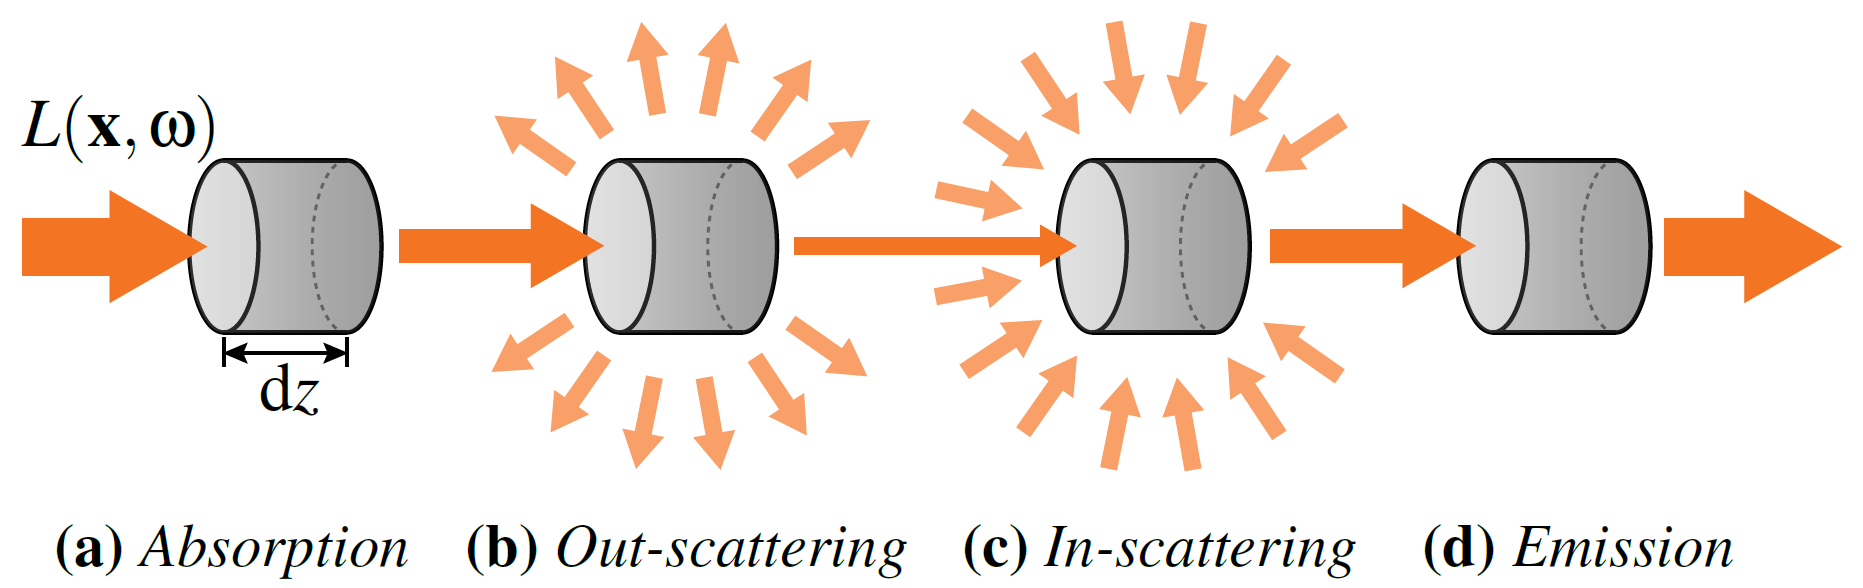
\includegraphics[width=0.7\linewidth]{img/novak_volume_effects.png}
    \caption[Physical effects in a volume]{The physical effects that are modeled by the \textit{radiative transfer equation} (Image from \cite{novak_overview}).}
    \label{fig:novak_volume_effects}
\end{figure}
These effects are quantified by the \textit{scattering coefficient} $\mu_s$ and the \textit{absorption coefficient} $\mu_a$ \cite{novak_overview}.
The sum of $\mu_s$ and $\mu_a$ is called the \textit{extinction coefficient} $\mu_t=\mu_a + \mu_s$ and accounts for either of the effects \cite{novak_overview}.
These coefficients are related with the density $\rho$ by the \textit{cross-sectional areas} $\sigma$ of the particles, thus for the scattering coefficient we have: $\mu_s = \rho \sigma_s$ \cite{novak_overview}.
We can further define the fraction of photons that scatter as the \textit{albedo} $\alpha=\frac{\mu_s}{\mu_t}$ \cite{novak_overview}.
With the integral form of the \textit{radiative transfer equation}, we have a way to formalize the scattering, emission and absorption of the medium \cite{novak_overview}:
\begin{equation}
    \begin{split}
        \label{eq:radiative_transfer}
        L(\boldsymbol{x}, \omega_o) = \int_0^\infty T(t)[\mu_a(\boldsymbol{y})L_e(\boldsymbol{y}, \omega_o) + \mu_s(\boldsymbol{y})L_s(\boldsymbol{y}, \omega_o)]dy & \;\text{with}\; \boldsymbol{y}=\boldsymbol{x} - y\omega_o \\
                                                                                                                                                                    & \;\text{and}\; t=||\boldsymbol{x}-\boldsymbol{y}||.
    \end{split}
\end{equation}
$T$ denotes the transmittance over the distance $t$ (Beer-Lambert law \cite{lambert}) and $L_s$ is the in-scattered radiance which accounts for the radiance scattered into the medium from all directions \cite{novak_overview}:
% \begin{multicols}{2}
% \end{multicols}
% \noindent\begin{minipage}{.5\linewidth}
% \end{minipage}
% \begin{minipage}{.5\linewidth}
% \end{minipage}
\begin{equation}
    \label{eq:beer_lambert_law}
    T(t) = e^{-\int_0^t \mu_t(\boldsymbol{x} - s\omega_o)ds},
\end{equation}
\begin{equation}
    \label{eq:in_scattered_radiance}
    L_s(\boldsymbol{x}, \omega_o) = \int_{\mathcal{S}^2} f_p(\omega_o, \omega_i)L_i(\boldsymbol{x}, \omega_i)d\omega_i.
\end{equation}
$f_p$ is called the \textit{phase function} and will be explained in Section \ref{subsec:phase_function}.

Now that we defined how light propagates in a medium, we can combine the formulation in Equation \ref{eq:radiative_transfer} with the surface formulation from equation \ref{eq:render_equation}.
We therefore clip the upper integration bound of equation \ref{eq:radiative_transfer} to a distance $z$ and add the attenuated surface term \cite{novak_overview}:
\begin{equation*}
    L(\boldsymbol{x}, \omega_o) = \int_0^z T(\boldsymbol{x}, \boldsymbol{y})[\mu_a(\boldsymbol{y})L_e(\boldsymbol{y}, \omega_o) + \mu_s(\boldsymbol{y})L_s(\boldsymbol{y}, \omega_o)]dy + T(\boldsymbol{x}, \boldsymbol{z})L(\boldsymbol{z}, \omega_o).
\end{equation*}
The idea of this \textit{volume rendering equation} is that a ray passing through a medium will hit a surface at distance $z$ \cite{novak_overview}.
The first part on the right side of this equation accounts for the in-scattering and emission of the medium while the second part represents absorbed or out-scattered radiance from the surface at distance $z$ \cite{novak_overview}.

\subsection{Solving the Beer-Lambert Law in Heterogeneous Media}
\label{subsec:solving_beer_lambert_law_in_heterogeneous_media}
As described in Section \ref{subsec:theory_of_light_propagation_in_participating_media} effects like scattering and absorption occur when light interacts with the particles of a medium.
We therefore need a way to sample interactions on which the light then is scattered or absorbed.
At distance $t$, the Beer-Lambert law from Equation \ref{eq:beer_lambert_law} gives us the proportion of light that did not hit a particle $P(X > t) = T(t)$ \cite{novak_overview}.
Therefore, we can compute the fraction of light that hit a particle by \cite{novak_overview}:
\begin{equation*}
    F(t) = 1 - T(t).
\end{equation*}
For a homogeneous medium the probability of hitting a particle is:
\begin{equation*}
    F(t) = 1 - e^{\mu_t t},
\end{equation*}
since $\mu_t$ is constant in the whole medium \cite{novak_overview}.
After rearranging, this gives us a method to sample free path distances in homogeneous media:
\begin{equation}
    \label{eq:distance_sampling}
    t(\xi) = -\frac{ln(1-\xi)}{\mu_t},
\end{equation}
where $\xi$ is a uniform random number in the interval $[0, 1)$ \cite{novak_overview}.

However, heterogeneous media distance sampling is more complex, since $\mu_t$ is no longer constant.
We could interpret each voxel as a homogeneous medium and sample a target transmittance in the interval $(0, 1]$ \cite{novak_overview}.
We then have to accumulate the transmittance over all voxels that a ray passes until it falls below the target transmittance \cite{novak_overview}.
This method is called \textit{regular tracking} \cite{sutton_regular_tracking}.
The drawback is, that we have to compute intersections with the voxels which can be expensive for detailed volumes \cite{novak_overview}.
Another approach is called \textit{ray marching} \cite{perlin_hypertexture}, where we traverse the medium at a constant step size.
Again, we accumulate the transmittance until it falls below a sampled target transmittance \cite{novak_overview}.
This method can reduce the cost compared to regular tracking but introduces bias, since it assumes a constant density between each step \cite{novak_overview}.
An unbiased approach that does not require intersection tests with voxels is \textit{Woodcock tracking} \cite{woodcock}, usually called \textit{delta tracking}.
Figure \ref{fig:novak_distance_sampling} visualizes all tree approaches.
\begin{figure}[ht]
    \centering
    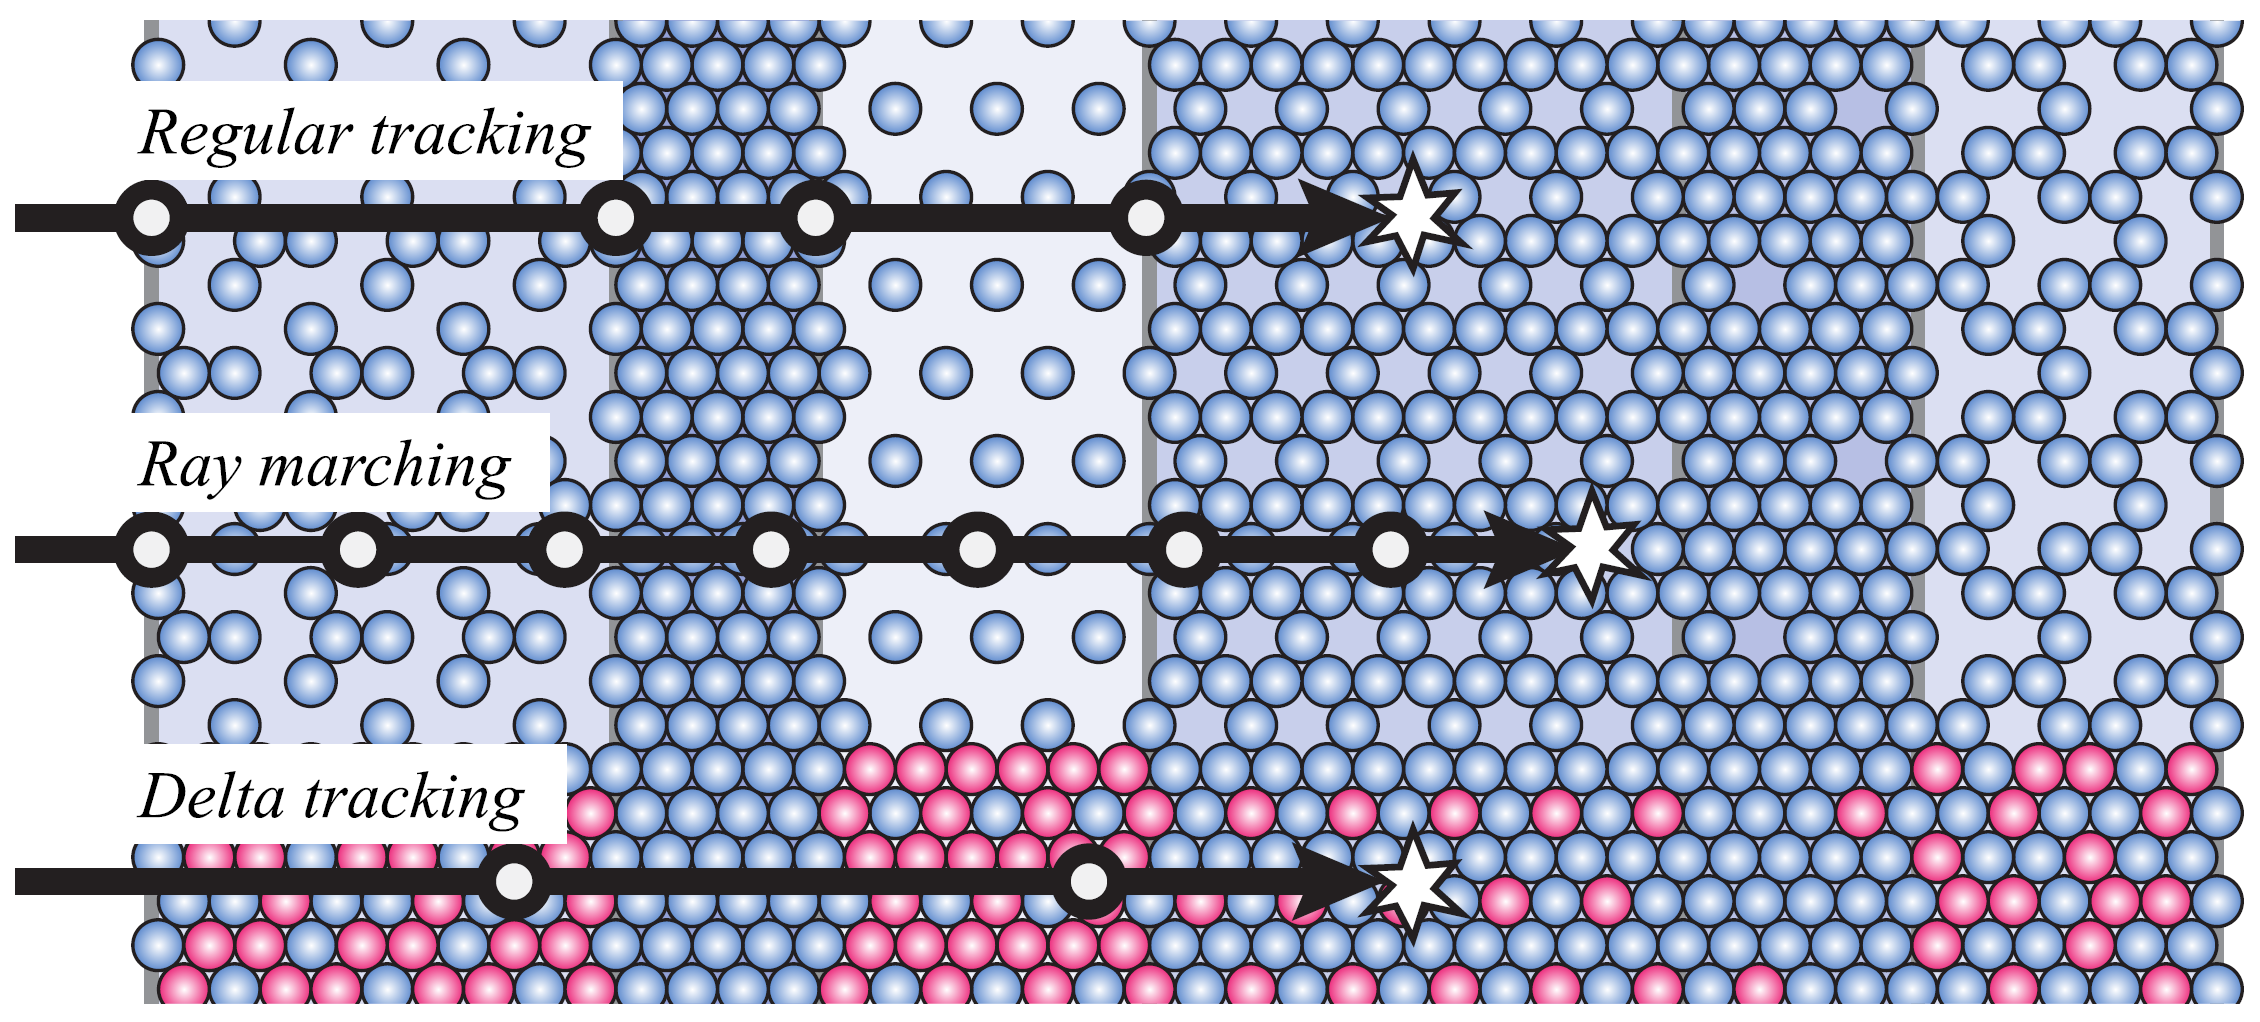
\includegraphics[width=0.7\linewidth]{img/novak_distance_sampling.png}
    \caption[Approaches for distance sampling in heterogeneous media]{Three approaches for distance sampling in heterogeneous media: Regular tracking gives exact results but requires intersections with voxel boundaries. Ray marching can reduce compute time but introduces a bias. For delta tracking we add fictious matter (red circles) to obtain a homogeneous medium and get an unbiased result (Image from \cite{novak_overview}).}
    \label{fig:novak_distance_sampling}
\end{figure}
We first have to homogenize the medium by adding fictious matter until the extinction reaches the majorant of the real matter $\bar{\mu_t}$ \cite{novak_overview}.
This fictious matter does not influence the scattering or absorption behavior \cite{novak_overview}.
We can then iteratively sample new distances using Equation \ref{eq:distance_sampling} with $\mu_t=\bar{\mu_t}$ and compare the local extinction coefficient $\mu_t(\boldsymbol{x})$ with the majorant $\bar{\mu_t}$ using a uniform random number $\xi\in[0,1)$ \cite{spectral_and_decomposition_tracking}.
If $\xi<\frac{\mu_t(\boldsymbol{x})}{\bar{\mu_t}}$ we found a hit with a particle and can exit the iteration, if $\xi>=\frac{\mu_t(\boldsymbol{x})}{\bar{\mu_t}}$ we found a null-collision meaning that we have to continue with sampling a new distance $t$ \cite{spectral_and_decomposition_tracking}.
Note that for a constant cross-sectional area $\sigma_t$ we can use the ratio between the local density $\rho(\boldsymbol{x})$ and the density majorant $\bar{\rho}$ instead.
To estimate the transmittance in a heterogeneous medium we employ a similar algorithm called \textit{ratio tracking} \cite{novak_ratio_tracking}.
As opposed to delta tracking, ratio tracking does not compare whether the interaction is a null-collision \cite{novak_ratio_tracking}.
Instead, it updates the transmission with $T_{new} = T_{old}(1 - \frac{\mu_t(\boldsymbol{x})}{\bar{\mu_t}})$ \cite{novak_ratio_tracking}.

Since both algorithms use a global majorant of the extinction, they perform poorly in media where the extinction varies strongly across the medium.
Therefore, we use local majorants as suggested by \citeauthor{brick_grid} \cite{brick_grid}.
This idea is visualized in Figure \ref{fig:brick_grid_majorants}.
\begin{figure}[ht]
    \centering
    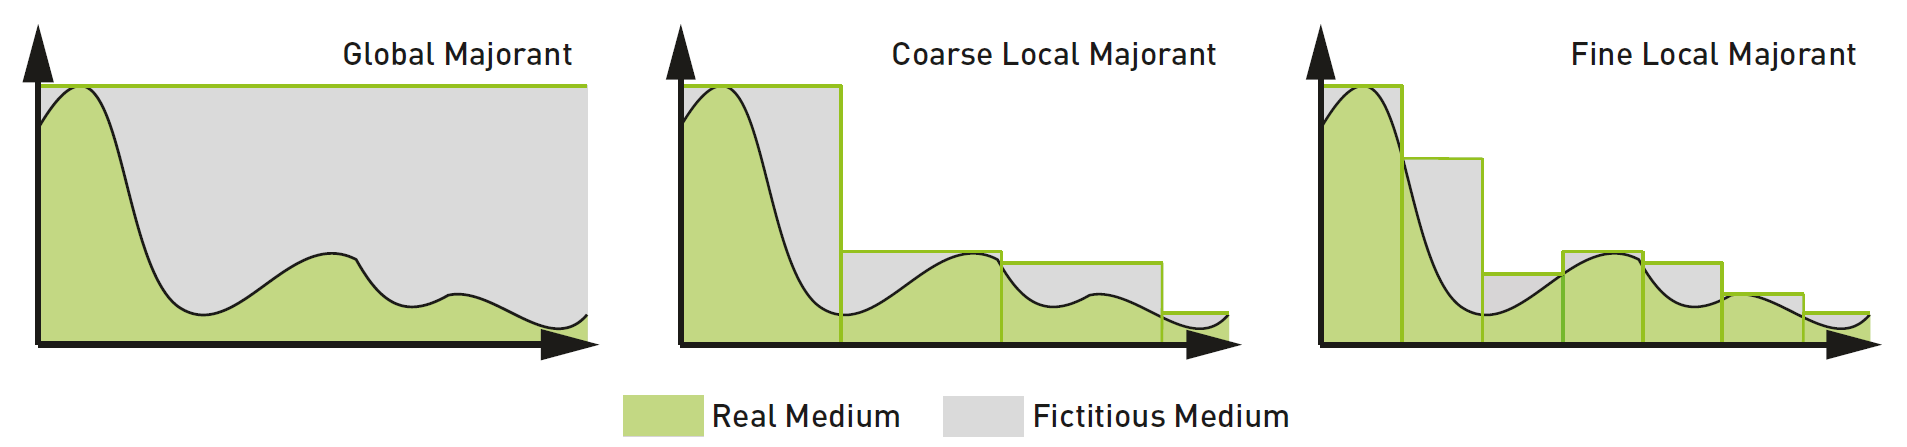
\includegraphics[width=0.9\linewidth]{img/brick_grid_majorants.png}
    \caption[Visualization of local density majorants]{Visualization of the concept of local majorants. These allow to sample distances and estimate transmittance more efficiently (Image from \cite{brick_grid}).}
    \label{fig:brick_grid_majorants}
\end{figure}
To store the volume data we use three textures.
First, we use an \textit{atlas texture} to store \textit{bricks} which are groups of $8 \times 8 \times 8$ voxels \cite{brick_grid}.
The second texture is the \textit{indirection texture} which stores offsets into the atlas.
This texture therefore links a position in space to a brick of data in the atlas \cite{brick_grid}.
Finally we store the minorant and majorant of each brick in the \textit{range texture} \cite{brick_grid}.
These are used to scale the density values in the atlas texture to the interval $[0, 1]$ \cite{brick_grid}.
The range texture additionally has three mipmap levels which allows to have local majorants at different scales \cite{brick_grid}.
Since the resulting atlas texture no longer has spatial coherence, hardware interpolation by the texture unit is not possible \cite{brick_grid}.
Therefore, we employ a form of stochastic lookup where we jitter the lookup point by $\pm0.5$ voxels before performing point sampling \cite{brick_grid}.
When having a large number of lookups, as it is the case in Monte Carlo integration, this procedure is equivalent to trilinear interpolation without introducing a significant overhead \cite{brick_grid}.
In Figure \ref{fig:brick_grid_datastructure} we show the introduced textures visually.
\begin{figure}[ht]
    \centering
    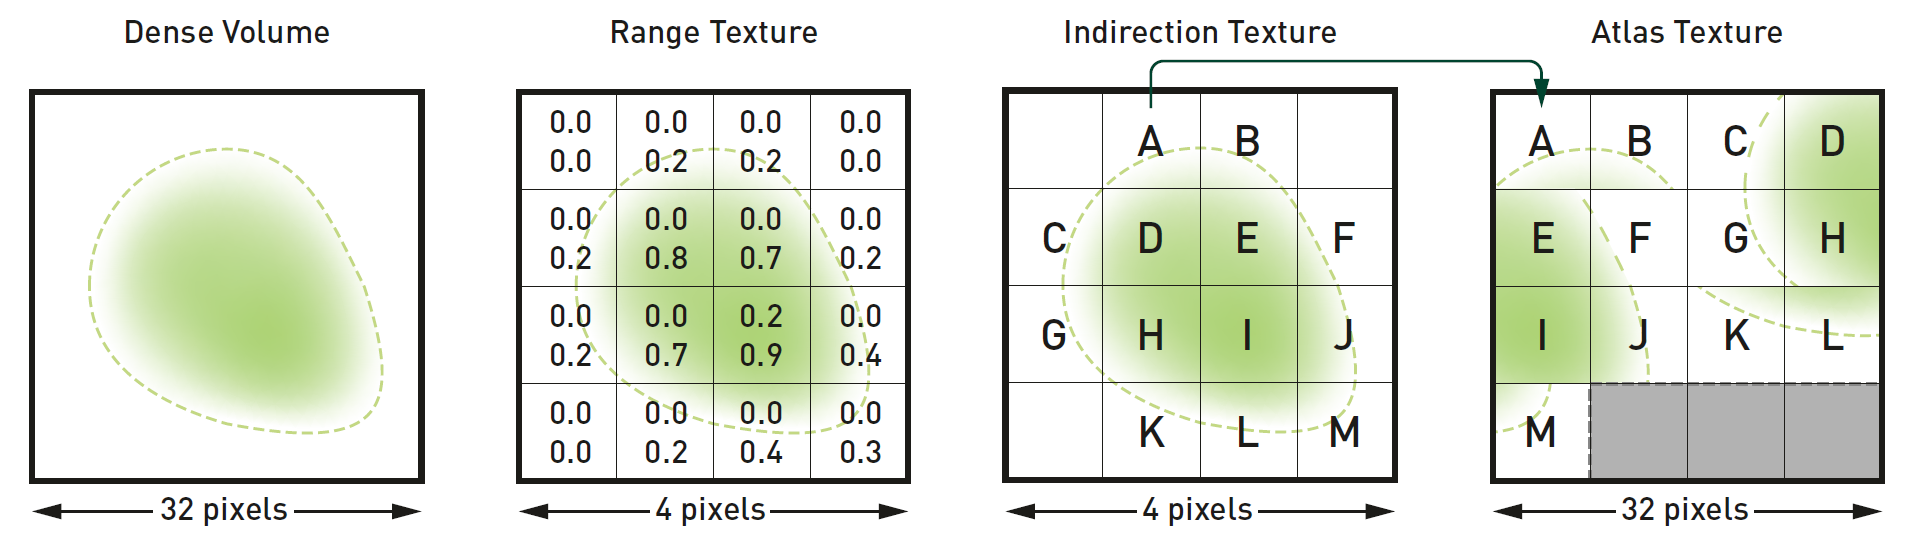
\includegraphics[width=0.9\linewidth]{img/brick_grid_datastructure.png}
    \caption[Data structure of brick grid]{Visualization of the internal data structure of brick grid. It uses a range texture, containing minorants and majorants and an indirection texture which links world positions to the density values in the atlas texture (Image from \cite{brick_grid}).}
    \label{fig:brick_grid_datastructure}
\end{figure}

For distance sampling and transmittance estimation we first sample a target optical thickness $\tau_{target}=-ln(1-\xi)$ \cite{brick_grid}.
We then accumulate the optical thicknesses of all bricks along a ray until the accumulated thickness exceeds the target thickness \cite{brick_grid}.
In this case we step back along the ray until it matches $\tau_{target}$ \cite{brick_grid}.
Now we perform the stochastic null-collision test by comparing the density at this point with the local majorant \cite{brick_grid}.
In the case of distance sampling, we return the distance to the first real collision \cite{brick_grid}.
For transmittance estimation, we adjust the current estimate by the ratio of real to fictious matter \cite{brick_grid}.
When having a null-collision, the algorithm is restarted by sampling a new target optical thickness \cite{brick_grid}.
This is repeated until a distance is successfully sampled, the transmittance estimation is stopped by Russian roulette or when the ray left the volume \cite{brick_grid}.

\subsection{Phase Functions}
\label{subsec:phase_function}
In Equation \ref{eq:in_scattered_radiance} the term of a \textit{phase function} was already introduced.
Now we want to explain this concept in more detail.
Similar like a \acs{brdf} gives the amount of light scattered into a certain direction on a surface, a phase function gives this amount in a volume when an interaction with a particle occurs \cite{novak_overview}.
As opposed to \acsp{brdf}, phase functions are normalized when they are integrated over the unit sphere $\mathcal{S}^2$, therefore they can be seen as \acsp{pdf} as well \cite{pbr}.
For the isotropic case, meaning that light is scattered in all directions with equal probability, we can ensure the normalization by dividing with the integration domain, which is $4\pi$ for the unit sphere \cite{pbr}.
This gives us the isotropic phase function \cite{novak_overview}:
\begin{equation*}
    f_p(\omega_o, \omega_i)=\frac{1}{4\pi}.
\end{equation*}
As it can be seen the function has a constant value for all directions $\omega_o$, $\omega_i$ on the unit sphere \cite{novak_overview}.

Since we want our \acp{lod} to look similar like the corresponding mesh representation, an isotropic phase function is not sufficient.
Instead, we choose the \acs{sggx} phase function \cite{sggx} because it provides scattering properties that match diffuse and specular \acsp{brdf}.
Particularly it is similar to microfacet models like the GGX \acs{brdf} \cite{ggx} which also led to the name \acf{sggx} \cite{sggx}.
The idea behind the GGX \ac{brdf} and other microfacet models is that a surface can be modeled by a distribution of normals which describe the roughness of the surface at a certain point \cite{ggx}.
Expanding on this idea \citeauthor{microflake} \cite{microflake} introduced the microflake framework which models the medium as two-sided specularly reflecting flakes which are distributed according to a certain \ac{ndf}.
\citeauthor{sggx} \cite{sggx} define the \ac{ndf} for the SGGX phase function as:
\begin{equation*}
    D(\omega_m)=\frac{1}{\pi \sqrt{|S|}(\omega_m^T S^{-1} \omega_m)^2},
\end{equation*}
where $\omega_m$ is the direction of the microflake normal and $S$ is a 3 $\times$ 3 symmetric positive definite matrix which encodes the scattering properties \cite{sggx}.
This matrix is computed from the GGX roughness value $\alpha$ and the normal $n$ of the surface it should represent as
\begin{equation*}
    S=\begin{pmatrix}x^2 & xy & xz \\ xy & y^2 & yz \\ xz & yz & z^2\end{pmatrix} + \alpha^2\begin{pmatrix}y^2 + z^2 & -xy & -xz \\ -xy & x^2+z^2 & -yz \\ -xz & -yz & x^2+y^2\end{pmatrix},
\end{equation*}
where $x$, $y$, $z$ are the components of the normal $n$ \cite{sggx}.
The \ac{ndf} $D(\omega_m)$ can be seen as the extension of the GGX \acs{ndf} to the negative hemisphere as Figure \ref{fig:sggx_ndf} shows.
\begin{figure}[ht]
    \centering
    \begin{subfigure}[b]{0.45\linewidth}
        \centering
        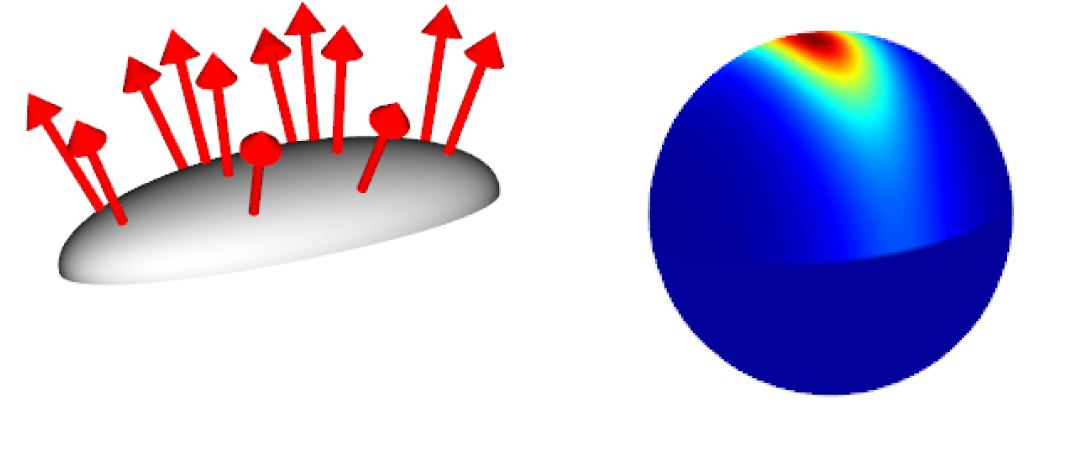
\includegraphics[width=\linewidth]{img/sggx_ndf_a.jpg}
        \caption{GGX $D(\omega_m), \omega_m \in \Omega^+$}
        \label{fig:sggx_ndf_a}
    \end{subfigure}
    \begin{subfigure}[b]{0.45\linewidth}
        \centering
        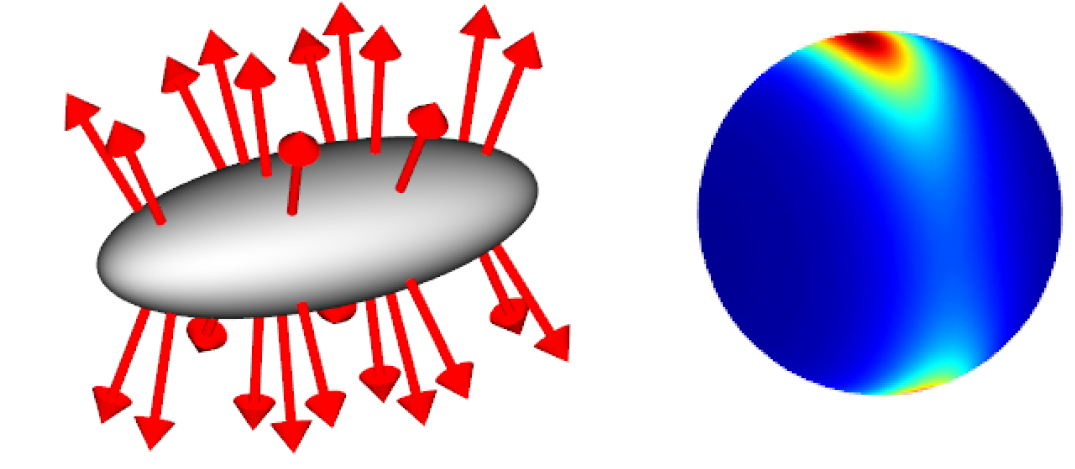
\includegraphics[width=1\linewidth]{img/sggx_ndf_b.jpg}
        \caption{SGGX $D(\omega_m), \omega_m \in \Omega$}
        \label{fig:sggx_ndf_b}
    \end{subfigure}
	\caption[Visualization of anisotropic \acsp{ndf}]{Visualization of anisotropic \acsp{ndf}. Note that the negative hemisphere of the SGGX \acs{ndf} is a mirroring of the positive hemisphere (Image from \cite{sggx}).}
	\label{fig:sggx_ndf}
\end{figure}
Based on the \acs{ndf} the authors then introduce a \ac{vndf} $D_{\omega_o}(\omega_m)$ which is used for importance sampling of the phase function, since it further reduces variance compared to the \acs{ndf} \cite{vndf_importance_sampling}.
Another important concept in the microflake framework is the projected area $\sigma(\omega_o)$ of the microflakes.
As depicted in Figure \ref{fig:sggx_projected_area}, this is the area of the microflakes when projected onto a plane in direction $\omega_o$ \cite{sggx}.
\begin{figure}[ht]
    \centering
    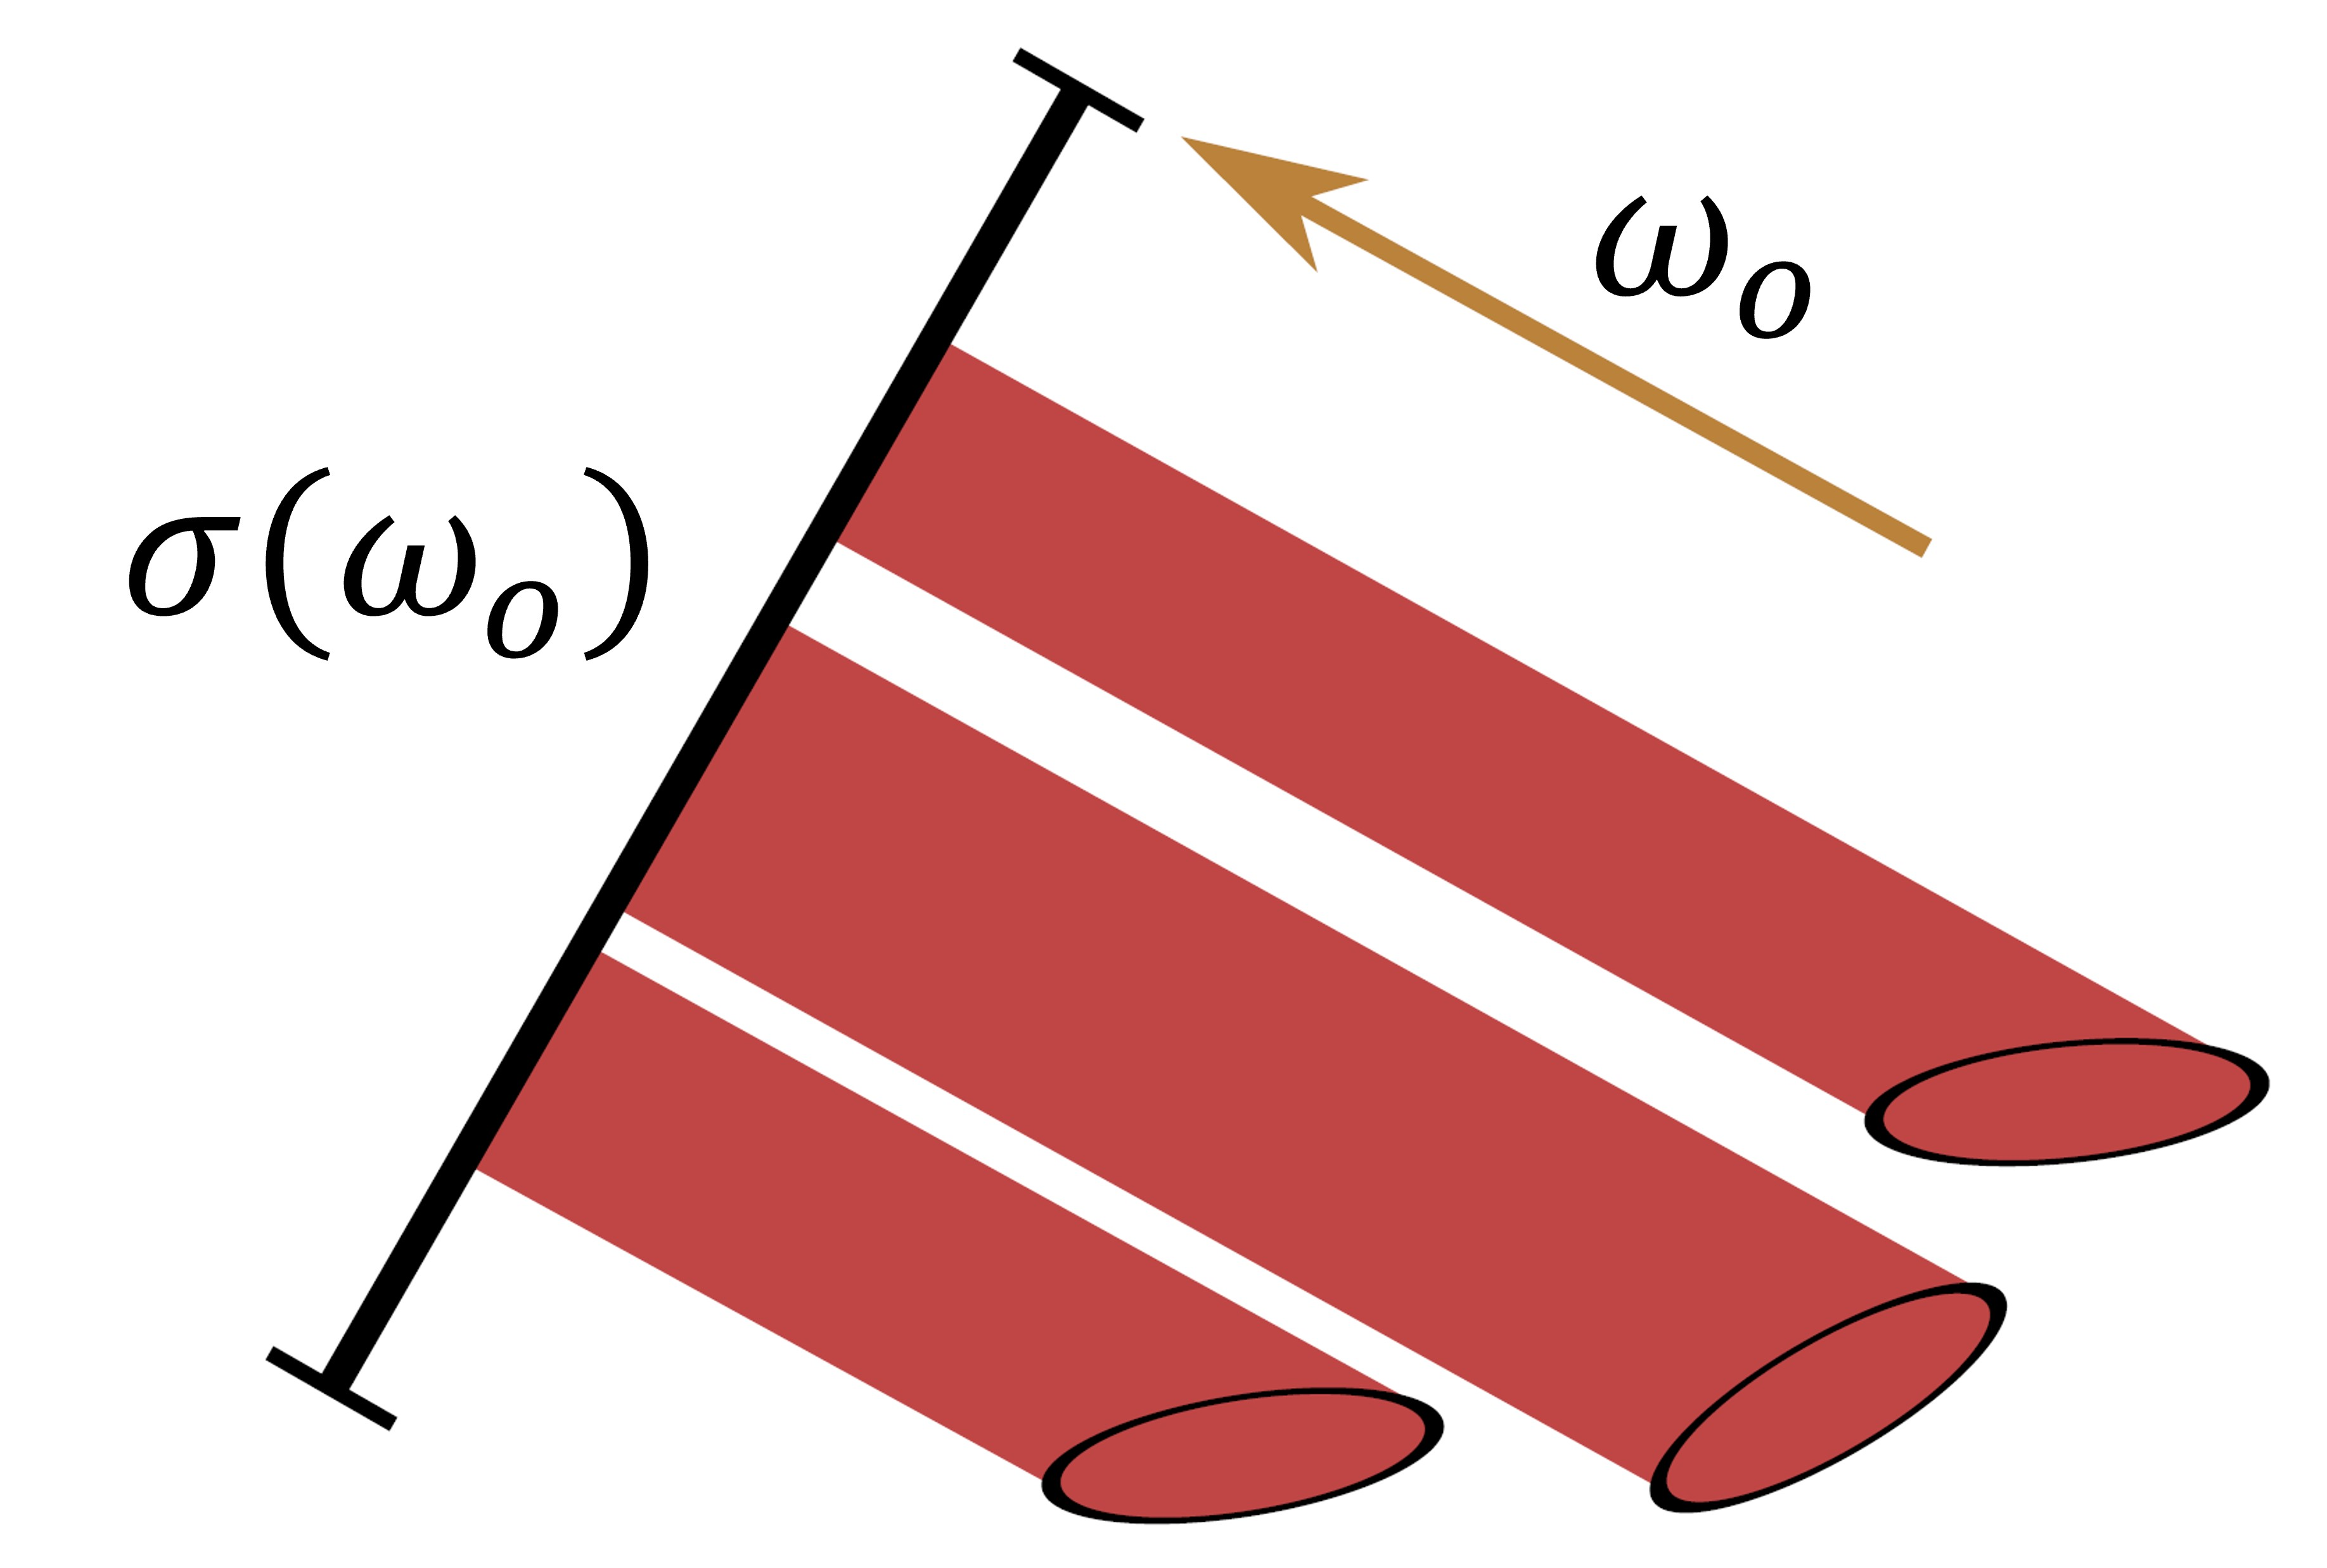
\includegraphics[width=0.3\linewidth]{img/sggx_projected_area.jpg}
    \caption[Illustration of the microflake projected area]{Illustration of the microflake projected area $\sigma(\omega_o)$, which is the area on a plane on which the microflakes are projected (Image from \cite{sggx}, with modification of the annotations).}
    \label{fig:sggx_projected_area}
\end{figure}
For the SGGX phase function the projected area is defined as \cite{sggx}:
\begin{equation}
    \label{eq:projected_area}
    \sigma(\omega_o)=\int_\Omega \langle \omega_o, \omega_m \rangle D(\omega_m) d\omega_m = \sqrt{\omega_o^T S \omega_o},
\end{equation}
where $\langle -,-\rangle$ denotes the clamped dot product \cite{sggx}.
Having defined these terms the authors introduce the actual phase function which consists of a specular and a diffuse component.
The specular component is evaluated as \cite{sggx}:
\begin{equation*}
    f{}^{spec}_p(\omega_o, \omega_i) = \frac{D(\omega_h)}{4 \sigma(\omega_o)}.
\end{equation*}
Importance sampling the specular component requires to sample a microflake normal $\omega_m$ from $D_{\omega_o}$ and the direction $\omega_o$ is reflected on this normal to generate an incident direction $\omega_i$ \cite{sggx}.
For evaluating the diffuse phase function the authors propose to sample a normal $\omega_m$ from $D_{w_o}$ which gives an unbiased estimate of the following integral \cite{sggx}:
\begin{equation*}
    f{}^{diff}_p(\omega_o, \omega_i) = \frac{1}{\pi}\int_\Omega \langle\omega_i,\omega_m\rangle D_{\omega_o}(\omega_m) d\omega_m = \lim \limits_{N \to +\infty} \frac{1}{N} \sum_{n=1}^N \frac{1}{\pi} \langle\omega_i,\omega_m(n)\rangle.
\end{equation*}
$f{}^{diff}_p$ can then be importance sampled by generating a direction $\omega_m$ from $D_{\omega_o}$ and then sampling the hemisphere given by $\omega_m$ \cite{sggx}.

\section{Transforming Meshes into Volumes}
\label{sec:transforming_meshes_into_volumes}
For generating \acp{lod} we need to transform the mesh representation into volumes.
We refer to this process as filtering.
% We follow the approach by \citeauthor{hybrid_mesh_volume_lods} and use ray casting to estimate the density for each voxel \cite{hybrid_mesh_volume_lods}.
We follow a similar approach as \citeauthor{hybrid_mesh_volume_lods} and use ray casting to estimate the density for each voxel \cite{hybrid_mesh_volume_lods}.
Our deviations from their approach are discussed in Section \ref{sec:mesh_filtering}.
To sample ray origins the authors use a \ac{pdf} $D_i=D_i^{cube} \ast D^{smooth}$ around the voxel center \cite{hybrid_mesh_volume_lods}.
$D_i^{cube}$ is a cubic uniform \ac{pdf} around the voxel center and $D^{smooth}$ is a 3D gaussian function with the standard deviation of 0.6 times the length of the voxel edge \cite{hybrid_mesh_volume_lods}.
The length of the rays is set to the length of the voxel edge \cite{hybrid_mesh_volume_lods}.
Each ray is intersected with the micro-geometry, the number of hits and the total number of rays casted determine the occlusion probability \cite{hybrid_mesh_volume_lods}:
\begin{equation*}
    P_{occ}=\frac{nbHits}{nbRays}.
\end{equation*}
Since a medium is defined on the density $\rho$ the authors solve the integral \cite{hybrid_mesh_volume_lods}:
\begin{equation}
    1 - \frac{1}{4\pi}\int_{\mathcal{S}^2} e^{-\rho\sigma(\omega)ray_l} d\omega = P_{occ}
    \label{eq:loubet_filtering_equation}
\end{equation}
for $\rho$ \cite{hybrid_mesh_volume_lods}.
$\sigma_u(\omega)$ is the microflake projected area as defined in Equation \ref{eq:projected_area} and $ray_l$ is again the length of the voxel edge \cite{hybrid_mesh_volume_lods}.
This equation cannot be solved analytically for the density and therefore requires gradient descent based optimization \cite{hybrid_mesh_volume_lods}.





